\chapter{State of the Art}
\label{ch:soa}

OMR has evolved through three broadly distinguishable generations: the
heuristic modular pipelines that defined the field from the 1990s through
the early 2010s; the convolutional--recurrent sequence models trained with
Connectionist Temporal Classification (CRNN--CTC) that arose with deep
learning; and the most recent end-to-end transformer architectures, which
scale to polyphonic and full-page input at the cost of substantially
larger labelled corpora.
This chapter surveys those paradigms, reviews the principal datasets and
symbolic output representations used in the literature, and finally
positions this thesis with respect to recent work that targets jazz lead
sheets specifically.
The two published surveys of the
field~\cite{calvoZaragozaUnderstandingOMR2020,shatriOPTICALMUSICRECOGNITION}
serve as the structural backbone for the discussion.

% ─────────────────────────────────────────────────────────────────────────────
\section{The Classical OMR Pipeline}
\label{sec:soa-classical}

Until the mid-2010s, almost every OMR system was a modular pipeline of four
sequential stages: image preprocessing (binarisation, deskewing); staff-line
detection and removal; segmentation and classification of the musical
primitives left behind once the staff lines have been erased; and semantic
reconstruction, in which the recognised primitives are assembled into a
structured score~\cite{calvoZaragozaUnderstandingOMR2020}.
\Cref{fig:soa-arch-bainbridge,fig:soa-arch-rebelo} show two
influential illustrations of this decomposition.
Both predate the deep-learning shift discussed in \Cref{sec:soa-crnn} and
share the same backbone of preprocessing, staff handling, primitive
recognition, and semantic reconstruction.

\begin{figure}[htbp]
  \centering
  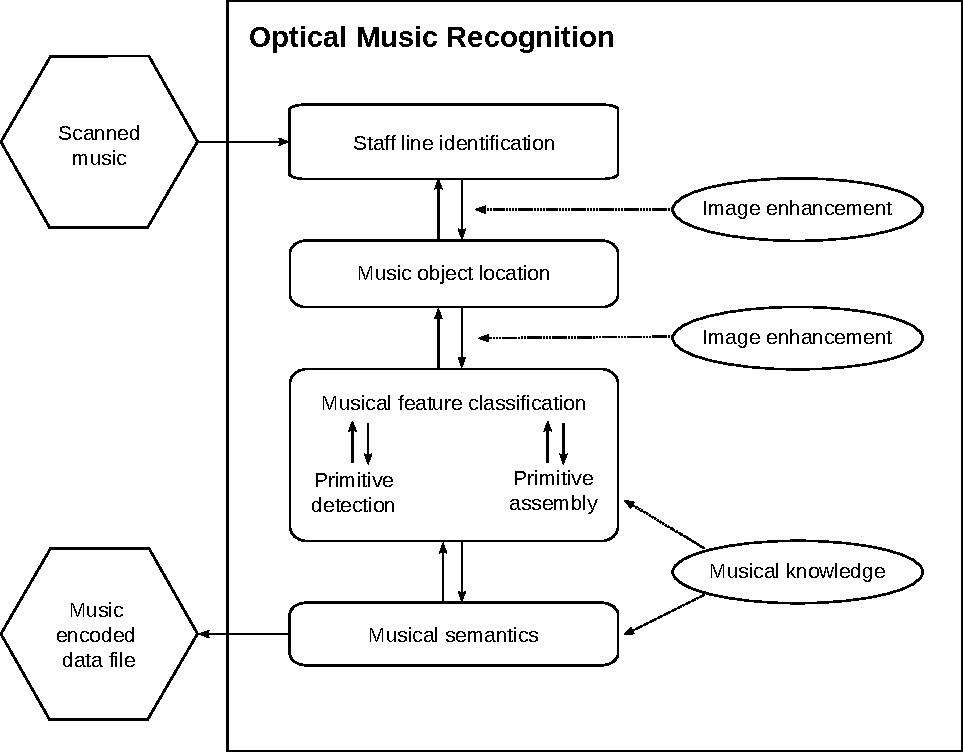
\includegraphics[width=0.82\textwidth]{figures/fig_omr_arch_bainbridge}
  \caption[Classical OMR pipeline (Bainbridge and Bell, 2001).]{Classical OMR
    pipeline architecture proposed by
    \textcite{bainbridgeChallengeOpticalMusic2001}. The four-stage structure
    (preprocessing, staff handling, primitive recognition, and semantic
    reconstruction) set the template for the field for two decades.
    Source: Wikimedia Commons, redrawn from the cited work.}
  \label{fig:soa-arch-bainbridge}
\end{figure}

\begin{figure}[htbp]
  \centering
  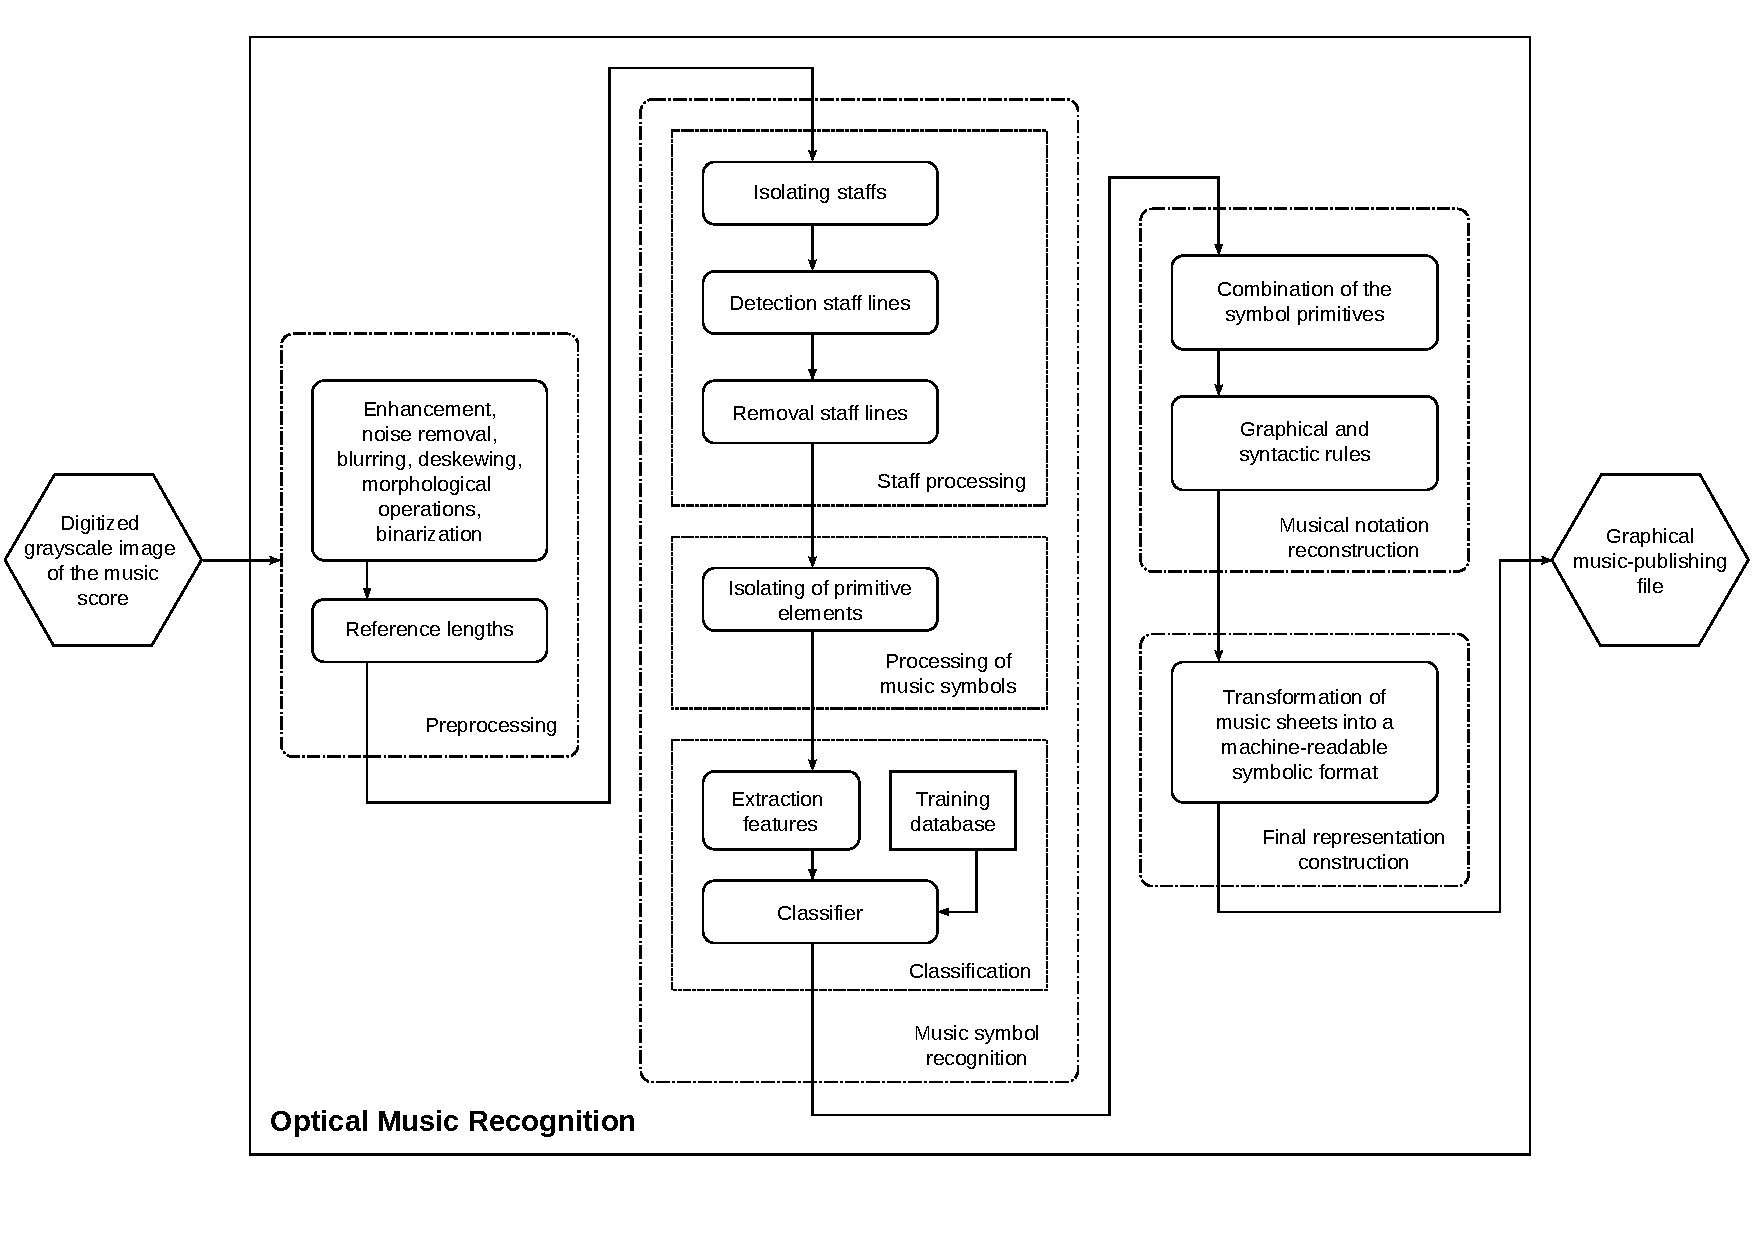
\includegraphics[width=0.82\textwidth]{figures/fig_omr_arch_rebelo}
  \caption[Classical OMR pipeline (Rebelo et al., 2012).]{The widely-cited
    OMR block diagram of \textcite{rebeloOpticalMusicRecognition2012}, which
    explicitly shows the feedback loops from musical knowledge into the
    recognition stages. Source: Wikimedia Commons, redrawn from the cited work.}
  \label{fig:soa-arch-rebelo}
\end{figure}

The second stage was historically the most studied because every subsequent
step depended on it.
Dalitz et al.~\cite{dalitzComparativeStudyStaff2008} compared the principal
families of staff-removal algorithms and contributed a skeletonisation-based
method; the \term{CVC-MUSCIMA} corpus~\cite{fornesCVCMUSCIMAGroundTruth2012}
was constructed expressly to benchmark this stage.

\term{Audiveris}~\cite{audiverisAudiveris} is the most widely deployed
open-source modular OMR engine.
Its processing chain combines morphological operations for staff and beam
handling, template matching for fixed-shape symbols, a small convolutional
classifier for ambiguous glyphs, and external OCR for lyrics, exporting
MusicXML~4.
The dominant commercial systems---SmartScore, PhotoScore, and
SharpEye---follow the same general decomposition but are
proprietary~\cite{calvoZaragozaUnderstandingOMR2020}.

Two structural weaknesses limit the modular approach for the input class
targeted in this thesis.
First, errors accumulate irreversibly across stages: a single missed staff
line corrupts every downstream pitch assignment for that staff, and a
mis-segmented chord symbol cannot be recovered by modules that have already
committed to a different reading.
Second, the visual heuristics that drive each module are tuned for classical
engraving styles; the rounded noteheads, loosely-spaced beams, and
hand-lettered chord symbols characteristic of \textit{The Real Book} fall
outside the operating envelope of the morphological filters those pipelines
rely on.
This motivates the move to learning-based, end-to-end recognition.

% ─────────────────────────────────────────────────────────────────────────────
\section{Deep Learning Paradigm: CRNN with CTC}
\label{sec:soa-crnn}

The deep-learning era of OMR begins with Calvo-Zaragoza and
Rizo~\cite{calvoZaragozaEndToEndNeural2018}, who in 2018 applied to
single-staff music the CRNN--CTC architecture that had recently become
standard for scene-text and handwritten-text recognition.
The model treats a staff image as a sequence of vertical strips, extracts
local visual features through a convolutional backbone, contextualises them
with a bidirectional recurrent network, and decodes the resulting per-frame
distribution into a token sequence using the CTC alignment---eliminating
the need for per-symbol segmentation.

Alongside the architecture, Calvo-Zaragoza and Rizo released the
\term{PrIMuS} corpus~\cite{PrIMuSDataset,calvoZaragozaEndToEndNeural2018}: 87\,678 real-music monophonic
incipits sourced from the RISM library and distributed in five
representations, including two purpose-built token formats.
The \term{agnostic} encoding lists visual primitives without musical
interpretation; the \term{semantic} encoding lists musical events such as
\code{note-C4\_eighth} or \code{keySignature-DM} directly.
The CRNN--CTC architecture trained on this corpus achieves Symbol Error
Rates near \SI{1}{\percent} on the agnostic encoding and the low single
digits on the semantic encoding, establishing the de facto baseline for
monophonic OMR.
A follow-up release---Camera-PrIMuS~\cite{calvoZaragozaCameraPrimus2018}---augments
the same incipits with synthetic photographic distortion and demonstrates
that the same network retains useful accuracy on phone-captured real-world
inputs.
This is the precise template that the present thesis follows.
\Cref{fig:soa-crnn-pipeline} illustrates the CRNN--CTC pipeline as applied
to a music staff.

\begin{figure}[htbp]
\centering
\begin{tikzpicture}[
  box/.style={
    draw, rounded corners=3pt,
    minimum width=1.6cm, minimum height=1.1cm,
    align=center, font=\small, text width=1.7cm,
    inner sep=3pt
  },
  arr/.style={->, thick, >=stealth},
  ann/.style={font=\scriptsize\itshape, text=black!55, align=center},
  node distance=0.45cm
]
  \node[box, fill=blue!8]      (img)  {Staff\\image};
  \node[box, fill=orange!18,   right=0.7cm of img]  (cnn)  {CNN\\backbone};
  \node[box, fill=teal!18,     right=0.7cm of cnn]  (lstm) {Bi-LSTM};
  \node[box, fill=violet!18,   right=0.7cm of lstm] (lin)  {Linear\\+\,softmax};
  \node[box, fill=red!10,      right=0.7cm of lin]  (ctc)  {CTC\\decoder};
  \node[box, fill=blue!8,      right=0.7cm of ctc]  (out)  {Token\\sequence};

  \draw[arr] (img)  -- (cnn);
  \draw[arr] (cnn)  -- (lstm);
  \draw[arr] (lstm) -- (lin);
  \draw[arr] (lin)  -- (ctc);
  \draw[arr] (ctc)  -- (out);

  \node[ann, below=0.2cm of cnn]  {feature column\\per time step};
  \node[ann, below=0.2cm of lstm] {contextualised\\hidden states};
  \node[ann, below=0.2cm of lin]  {per-frame vocab\\distribution};
  \node[ann, below=0.2cm of ctc]  {blank-collapsed\\tokens};
\end{tikzpicture}
\caption[CRNN--CTC pipeline for monophonic OMR.]{%
  The CRNN--CTC pipeline applied to a music staff.
  The image is treated as a sequence of vertical feature columns extracted
  by a convolutional backbone (ResNet18 in this work); a bidirectional LSTM
  contextualises each column; a linear projection produces a per-frame
  probability distribution over the vocabulary; and CTC decoding collapses
  the blank-padded alignment into a flat token sequence---without requiring
  any explicit symbol segmentation.
  Architecture introduced by \textcite{calvoZaragozaEndToEndNeural2018}.}
\label{fig:soa-crnn-pipeline}
\end{figure}

% ─────────────────────────────────────────────────────────────────────────────
\section{End-to-End Transformer Architectures}
\label{sec:soa-transformer}

From 2024 onward the OMR community has converged on attentional
encoder--decoder transformers for tasks that exceed the scope of monophonic
single-staff recognition.
The \term{Sheet Music Transformer}
(SMT)~\cite{riosVilaSheetMusicTransformer2024} was the first fully
transformer-based image-to-sequence OMR system to address polyphonic
transcription end-to-end: a vision-transformer encoder produces a flattened
patch sequence which a stacked decoder autoregressively maps to the
linearised target representation, dispensing with CTC entirely.
\term{SMT++}~\cite{riosVilaSMTPlusPlus2024} extends the approach to
full-page pianoform input and currently defines the state of the art on
that task.
\term{LEGATO}~\cite{yangLEGATO2025}---released in mid-2025---takes the
trend further with a vision-LLM backbone, an ABC-notation decoder, and over
214\,000 typeset pages of pretraining, reporting absolute error reductions
of \SI{47}{\percent}--\SI{68}{\percent} over previous state of the art on
hard typeset benchmarks.

\Cref{fig:soa-transformer-pipeline} shows the generic encoder--decoder
structure shared by these systems.

\begin{figure}[htbp]
\centering
\begin{tikzpicture}[
  box/.style={
    draw, rounded corners=3pt,
    minimum width=1.9cm, minimum height=1.1cm,
    align=center, font=\small, text width=2.0cm,
    inner sep=4pt
  },
  wide/.style={
    draw, rounded corners=3pt,
    minimum width=2.7cm, minimum height=1.1cm,
    align=center, font=\small, text width=2.8cm,
    inner sep=4pt
  },
  arr/.style={->, thick, >=stealth},
  darr/.style={->, thick, >=stealth, dashed, black!45},
  lbl/.style={font=\scriptsize\itshape, text=black!55, align=center}
]
  %% ── Encoder row ──────────────────────────────────────────────────
  \node[box,  fill=orange!12]                    (img) {Sheet music\\image};
  \node[wide, fill=orange!22, right=0.9cm of img](enc) {Vision Transformer\\Encoder (ViT)};
  \node[box,  fill=gray!14,   right=0.9cm of enc](mem) {Context\\memory};

  \draw[arr] (img) -- (enc);
  \draw[arr] (enc) -- (mem);

  %% ── Decoder row — 3.0 cm below encoder centres ───────────────────
  \node[box,  fill=green!12,  below=3.0cm of img] (prev)
      {\texttt{<SOS>} +\\prev.\ tokens};
  \node[wide, fill=green!22, right=0.9cm of prev] (dec)
      {Autoregressive\\Transformer Decoder};
  \node[box,  fill=blue!10,  right=0.9cm of dec]  (nxt) {Next\\token};

  \draw[arr] (prev) -- (dec);
  \draw[arr] (dec)  -- (nxt);

  %% ── Cross-attention ──────────────────────────────────────────────
  %% mem.south → drop 1.0 cm (corner) → left → dec.north
  \coordinate (ca-corner) at ($(mem.south) + (0,-1.0)$);
  \draw[arr, blue!65, line width=1.1pt]
      (mem.south) -- (ca-corner) -| (dec.north);
  %% Label sits above the horizontal segment, centred between mem and dec
  \node[lbl, text=blue!65, above=3pt]
      at ($(ca-corner)!0.5!(dec.north |- ca-corner)$) {cross-attention};

  %% ── Autoregressive feedback ──────────────────────────────────────
  %% nxt.south → drop 0.65 cm → left → prev.south (U-shape below all)
  \draw[darr]
      (nxt.south)  -- ++(0,-0.65)
      -- ($(prev.south) + (0,-0.65)$)
      -- (prev.south);
  %% Label below the horizontal segment, centred between prev and nxt
  \node[lbl] at ($(nxt.south)!0.5!(prev.south) + (0,-1.05)$)
      {autoregressive (step $t \to t\!+\!1$)};

\end{tikzpicture}
\caption[Encoder--decoder transformer architecture for OMR (SMT style).]{%
  The encoder--decoder transformer used in OMR systems such as
  SMT~\cite{riosVilaSheetMusicTransformer2024} and
  SMT++~\cite{riosVilaSMTPlusPlus2024}.
  A Vision Transformer (ViT) encoder maps the sheet music image to a
  sequence of patch embeddings; an autoregressive decoder then generates
  the output token sequence one token at a time, attending at each step to
  the full encoder memory via cross-attention.
  Unlike CRNN--CTC, no explicit segmentation or conditional-independence
  assumption is imposed---the decoder can, in principle, model arbitrary
  long-range token dependencies.}
\label{fig:soa-transformer-pipeline}
\end{figure}

These architectures, however, demand resources that exceed the budget of
a Bachelor's thesis.
For a strictly monophonic target domain---where the CRNN--CTC baseline
already attains sub-percent SER and the headroom for further gain is in
domain robustness rather than model capacity---CRNN--CTC remains the right
point on the cost/capability curve.
The quantitative justification of this choice is developed in
\Cref{ch:mgmt}.

% ─────────────────────────────────────────────────────────────────────────────
\section{Datasets for OMR Training}
\label{sec:soa-datasets}

The choice of architecture is inseparable from the choice of training
corpus.
\Cref{tab:omr-datasets} summarises the principal labelled corpora
available to the field as of 2026.

\begin{table}[htbp]
\centering
\small
\setlength{\tabcolsep}{5pt}
\renewcommand{\arraystretch}{1.35}
\begin{tabularx}{\textwidth}{@{} l L L L L @{}}
\toprule
\textbf{Dataset} & \textbf{Type} & \textbf{Size} & \textbf{Labels} & \textbf{Use} \\
\midrule
PrIMuS~\cite{PrIMuSDataset,calvoZaragozaEndToEndNeural2018} & Monophonic, typeset  & 87\,678 incipits                       & agnostic / semantic / MEI  & Monophonic CRNN--CTC training \\ \tfgrowsep
Camera-PrIMuS~\cite{calvoZaragozaCameraPrimus2018} & Monophonic, distorted        & 87\,678 incipits                       & same as PrIMuS             & Domain-robustness training \\ \tfgrowsep
DeepScoresV2~\cite{tuggenerDeepScoresV22020}      & Polyphonic, typeset           & 255\,385 pages, $\sim$151\,M symbols   & per-symbol bboxes + masks  & Music object detection \\ \tfgrowsep
CVC-MUSCIMA~\cite{fornesCVCMUSCIMAGroundTruth2012} & Polyphonic, handwritten      & 1\,000 pages                           & staff-removal masks        & Staff removal / writer ID \\ \tfgrowsep
MUSCIMA++~\cite{hajicMuscimaPP2017}               & Polyphonic, handwritten       & 140 pages, $\sim$91\,k symbols         & MuNG notation graph        & Symbol + relation recognition \\ \tfgrowsep
DoReMi~\cite{shatriDoReMi2021}                    & Polyphonic, typeset (Dorico)  & $\sim$6\,432 pages, $\sim$1\,M objects\todo{verify: exact page and object counts from DoReMi arXiv 2107.07786} & MusicXML + MuNG-style      & Universal OMR research \\ \tfgrowsep
OLiMPiC~\cite{mayerPracticalEndToEnd2024}         & Pianoform, typeset + scan     & $\sim$17\,945 synth, 2\,931 scanned\todo{verify: confirm split counts against Mayer et al. 2024 Table 1}    & MusicXML / LMX             & End-to-end pianoform OMR \\
\bottomrule
\end{tabularx}
\caption{Principal labelled corpora used in modern OMR research.
PrIMuS is the only one specifically designed for monophonic single-staff
training; it is the foundation of the synthetic dataset constructed in
this work.}
\label{tab:omr-datasets}
\end{table}

Two observations shape the data strategy of this thesis.
First, none of these corpora captures the LilyJAZZ-style engraving of
\textit{The Real Book}, and none labels chord symbols as first-class
objects; the only directly comparable corpus emerged contemporaneously
with this work~\cite{martinezSevillaJazzLeadSheets2025} and remains too
small to train a CRNN--CTC model from scratch.
Second, every recent end-to-end system---SMT, SMT++, OLiMPiC, LEGATO, and
Camera-PrIMuS itself---follows the same recipe of synthetic pretraining
followed by fine-tuning on a small annotated target set.
This is the recipe applied here.

% ─────────────────────────────────────────────────────────────────────────────
\section{Symbolic Output Representations}
\label{sec:soa-representations}

The output of an OMR system is a symbolic description of the score; the
choice of representation shapes both the modelling architecture and the
achievable error rate.
\textbf{MusicXML} is the de facto interchange standard between notation
editors and preserves polyphony, layout, lyrics, and chord symbols
losslessly, but its verbosity inflates sequence length and vocabulary size
when fed to a sequence model.
\textbf{MEI} is even more expressive but inherits the same penalty.
\textbf{Humdrum} \code{**kern} and \textbf{ABC notation} are far more
compact and are used as targets of recent
transformer-based work~\cite{riosVilaSheetMusicTransformer2024,yangLEGATO2025},
at the cost of reduced expressiveness for complex multi-voice layout.
The PrIMuS \textbf{agnostic} and \textbf{semantic} formats are compact and
CTC-friendly but interoperate only with the PrIMuS ecosystem.

\textbf{LMX} (Linearised MusicXML), introduced by
Mayer et al.~\cite{mayerPracticalEndToEnd2024} and maintained as an open
specification~\cite{OMRResearchLmx2025}, depth-first-traverses the
MusicXML tree and emits one whitespace-separated token per leaf event.
It is round-trippable to MusicXML with minimal information loss,
substantially more compact than the parent format, and was designed
specifically as a CRNN- and transformer-friendly target; the OLiMPiC
reference implementation provides a Python \code{Linearizer}/\code{Delinearizer}
pair that converts between the two representations directly.

This work adopts LMX with a project-specific grammar that drops features
outside the jazz lead-sheet domain (tuplets, slurs, articulations, double
accidentals, non-treble clefs); the full grammar is described in
\Cref{sec:lmx-format}.
LMX was preferred over the PrIMuS native formats because it round-trips
losslessly to MusicXML---the format expected by downstream music
applications---and because using the same representation as the OLiMPiC
reference work~\cite{mayerPracticalEndToEnd2024} keeps the present results
directly comparable.

% ─────────────────────────────────────────────────────────────────────────────
\section{Evaluation Metrics}
\label{sec:soa-metrics}

\textbf{Symbol Error Rate} (SER) is the de facto evaluation metric for
sequence-based OMR.
It is defined as the Levenshtein edit distance between the predicted and
the reference token sequences, normalised by the reference
length~\cite{SymbolErrorRate}, mirroring the Word Error Rate of automatic
speech recognition.
Its principal weaknesses, flagged by both Shatri and
Fazekas~\cite{shatriOPTICALMUSICRECOGNITION} and by Hajič et
al.~\cite{hajicOMRMetricsEvaluation2019}, are that all token-level edits
count equally regardless of musical significance and that SER values
depend on the chosen tokenisation, so they are not directly comparable
across encodings.

Two recent metrics partially address these shortcomings.
\textbf{TEDn} (normalised tree edit distance on the parsed MusicXML tree)
weights structural errors appropriately and is the primary metric in
OLiMPiC and SMT++.
\textbf{OMR-NED}~\cite{martinezSevillaOMRNED2025} extends SER with
per-element categories so that error distribution---not only error
rate---is legible from the metric itself.
This thesis reports SER as the primary metric for backward comparability
and complements it with a category-level error breakdown in
\Cref{ch:results}.

% ─────────────────────────────────────────────────────────────────────────────
\section{OMR for Jazz Lead Sheets}
\label{sec:soa-jazz}

Despite the cultural importance of jazz fake-books, OMR of jazz lead sheets
received almost no dedicated attention in the published literature before
2025.
Both major surveys~\cite{calvoZaragozaUnderstandingOMR2020,shatriOPTICALMUSICRECOGNITION}
list chord-symbol handling among the gaps in the field, and no
general-purpose OMR engine treats chord symbols as a first-class output
class.

The earliest dedicated work is an undergraduate honours thesis at
UCF~\cite{reedHonorsLeadSheets2018}, which built a non-deep modular
pipeline for chord-symbol recognition on printed and handwritten lead
sheets and used the recovered chord progressions to attempt
formal-structure reconstruction.
The closest published precedent is
\textbf{Martínez-Sevilla et al.}~\cite{martinezSevillaJazzLeadSheets2025},
presented at ISMIR 2025 and roughly contemporaneous with the final stages
of this thesis.
That work introduces a 293-sheet dataset of \textit{handwritten} jazz lead
sheets with \code{**kern} and MusicXML ground truth, and trains a
transformer-decoder model with symbolic-aware tokenisation, pretrained on
synthetic data and fine-tuned on the handwritten target set.

The present work differs in input domain (printed and scanned Real Book
pages versus fully handwritten sheets), in architecture (CRNN--CTC versus
transformer decoder), in chord handling (a two-stream design with
independent staff and chord networks merged in post-processing versus a
unified single-stream model), and in output format
(LMX versus \code{**kern}).
The two systems are thus complementary points in the design space, and
both contribute training corpora, models, and evaluation protocols that
future work can compare and combine.

% ─────────────────────────────────────────────────────────────────────────────
\section{Summary}
\label{sec:soa-summary}

Modular pipelines remain useful for full-page typeset classical scores but
do not generalise to the visual and semantic peculiarities of jazz lead
sheets.
End-to-end deep models---CRNN--CTC for monophonic input, transformers for
polyphonic and full-page input---now define the methodological frontier
and converge on a common recipe of synthetic pretraining followed by
fine-tuning on a small annotated target set.
Symbolic output formats have moved toward MusicXML-linear encodings
(prominently LMX), and evaluation practice is gradually shifting from raw
SER toward structurally aware metrics.
Jazz lead-sheet OMR remained essentially open until 2025; this thesis and
the concurrent ISMIR 2025
work~\cite{martinezSevillaJazzLeadSheets2025} represent the first two
focused attempts to fill that niche.
The architectural choices made in this thesis---detailed in
\Cref{ch:design}---are motivated by the findings surveyed above.
